% ============================================================
% CHƯƠNG 2: ỨNG DỤNG — THỰC NGHIỆM TRÊN BỐN BÀI TOÁN
% ============================================================
\chapter{Ứng dụng: Thực nghiệm trên Bốn Bài toán}
\label{chap:ung-dung}

Chương này trình bày việc áp dụng các nguyên lý đã trình bày ở
Chương~\ref{chap:co-so-ly-thuyet} vào bốn nhóm bài toán cụ thể. Mỗi
nhóm sử dụng một cách mã hóa khác nhau: tối ưu không ràng buộc dùng mã
hóa số thực (Mục~\ref{sec:ud-khong-rang-buoc}), tối ưu có ràng buộc
cũng dùng mã hóa số thực nhưng kết hợp thêm cơ chế xử lý ràng buộc
(Mục~\ref{sec:ud-co-rang-buoc}), bài toán người du lịch dùng mã hóa
hoán vị (Mục~\ref{sec:ud-tsp}), và hồi quy ký hiệu dùng mã hóa dạng cây
biểu thức theo nguyên lý Lập trình Di truyền
(Mục~\ref{sec:ud-symbolic-regression}). Với mỗi bài toán, phát biểu
toán học đầy đủ được trình bày trước, sau đó là phương pháp so sánh
được sử dụng và bảng kết quả thực nghiệm.

\section{Tối ưu không ràng buộc}
\label{sec:ud-khong-rang-buoc}

Năm hàm benchmark kinh điển của tối ưu không ràng buộc được sử dụng để
đánh giá khả năng tìm cực trị toàn cục của GA. Cả năm hàm đều có hai
biến $x, y$ và một cực tiểu toàn cục đã biết trước, cho phép so sánh
trực tiếp giá trị GA tìm được với giá trị đúng. Việc chọn đúng năm hàm
này không ngẫu nhiên: mỗi hàm đại diện cho một kiểu địa hình gây khó
khăn khác nhau, nhờ đó bộ năm hàm bao quát được các tình huống mà một
thuật toán tối ưu toàn cục phải đối mặt. Với mỗi hàm, đồ thị hàm trong không
gian ba chiều và đường hội tụ thực nghiệm của GA được đặt lần lượt
trong cùng một hình, để đối chiếu giữa đặc điểm địa hình và hành vi
hội tụ tương ứng.

\textbf{Hàm Easom} có công thức
\begin{equation}
f(x,y) = -\cos(x)\cos(y)\exp\!\left(-(x-\pi)^2-(y-\pi)^2\right),
\qquad x, y \in [-100,\, 100],
\label{eq:easom}
\end{equation}
với cực tiểu toàn cục $f(\pi,\pi) = -1$. Khó khăn của hàm này nằm ở
chỗ thừa số $\exp(-(x-\pi)^2-(y-\pi)^2)$ tắt cực nhanh khi rời khỏi
điểm $(\pi,\pi)$: chỉ cần cách tâm khoảng ba đơn vị, giá trị hàm đã
nhỏ hơn $10^{-4}$ và coi như bằng $0$. Vùng thực sự mang thông tin
dẫn đường vì thế chiếm chưa tới $0{,}1\%$ diện tích miền tìm kiếm
$[-100,100]^2$, toàn bộ phần còn lại là một mặt phẳng gần như tuyệt
đối. Đây là tình huống bất lợi nhất cho mọi phương pháp dựa trên
gradient: đứng ở vùng phẳng thì đạo hàm xấp xỉ $0$ theo mọi hướng, nên
không có thông tin cục bộ nào chỉ ra nên đi về đâu. Hàm này vì vậy
kiểm tra thuần túy khả năng \textit{tìm ra} đúng vùng chứa nghiệm bằng
cách rải điểm, chứ không phải khả năng tinh chỉnh.

\begin{figure}[htbp]
\centering
\begin{subfigure}[b]{0.72\linewidth}
    \centering
    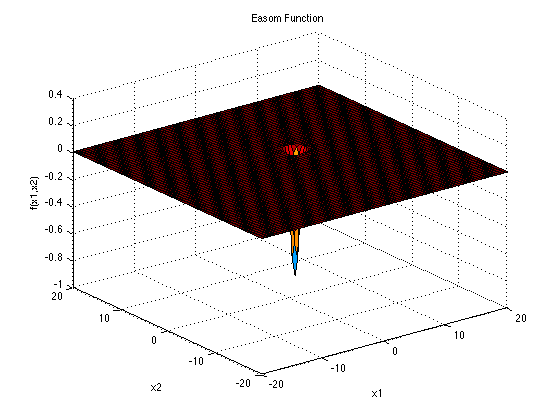
\includegraphics[width=\linewidth]{figures/easom.png}
    \caption{Hàm Easom trong không gian ba chiều}
\end{subfigure}

\vspace{0.8em}

\begin{subfigure}[b]{0.72\linewidth}
    \centering
    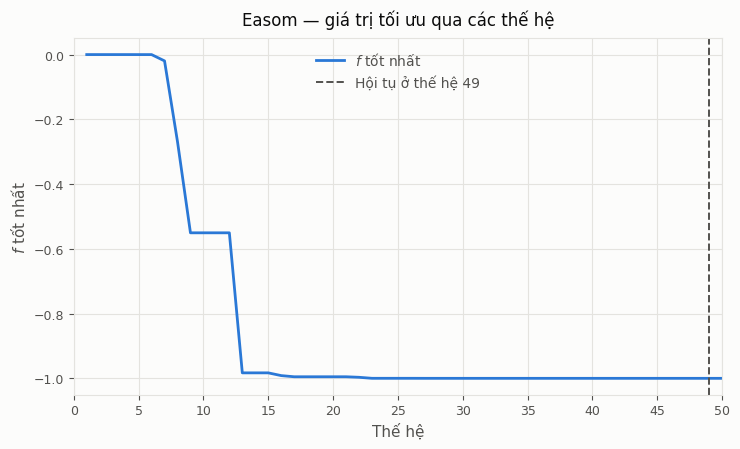
\includegraphics[width=\linewidth]{figures/hoitu_easom.png}
    \caption{Đường hội tụ của GA}
\end{subfigure}
\caption{Hàm Easom: đồ thị trong không gian ba chiều và diễn biến giá trị
tốt nhất qua các thế hệ. Đường nét đứt đánh dấu thế hệ mà GA chốt được
nghiệm tốt nhất.}
\label{fig:easom}
\end{figure}

\textbf{Hàm Rastrigin} có công thức
\begin{equation}
f(x,y) = 20 + x^2 + y^2 - 10\cos(2\pi x) - 10\cos(2\pi y),
\qquad x, y \in [-5.12,\, 5.12],
\label{eq:rastrigin}
\end{equation}
với cực tiểu toàn cục $f(0,0) = 0$. Hai số hạng cosin có chu kỳ bằng
$1$ nên tạo ra một mạng lưới cực tiểu cục bộ nằm xấp xỉ tại các điểm
có tọa độ nguyên; trong miền $[-5.12,\, 5.12]^2$ có khoảng $121$ cực
tiểu cục bộ như vậy, bao quanh dày đặc cực tiểu toàn cục tại gốc tọa
độ. Khó khăn ở đây là bài toán \textit{đa cực trị} điển hình: một
phương pháp cục bộ xuất phát từ điểm ngẫu nhiên gần như chắc chắn rơi
vào giếng gần nhất rồi dừng lại, và giếng đó hầu như không bao giờ là
giếng ở gốc tọa độ. Cái cứu GA ở đây là biên độ đột biến: với
$\sigma = 0{,}08 \times 10{,}24 \approx 0{,}82$, một bước đột biến đủ
lớn để nhảy qua vài ô lưới cực tiểu cục bộ (khoảng cách giữa hai giếng
liền kề là $1$), nên cá thể không bị giam trong một giếng duy nhất.

\begin{figure}[htbp]
\centering
\begin{subfigure}[b]{0.72\linewidth}
    \centering
    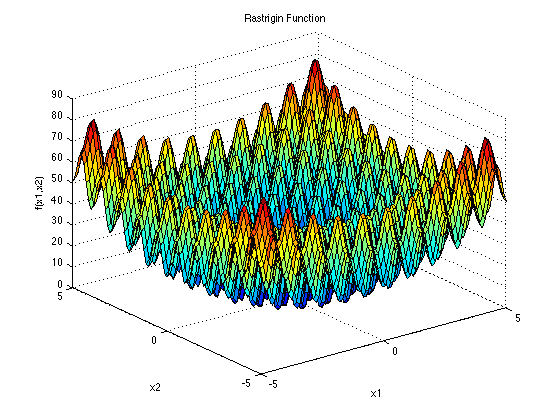
\includegraphics[width=\linewidth]{figures/rastrigin.png}
    \caption{Hàm Rastrigin trong không gian ba chiều}
\end{subfigure}

\vspace{0.8em}

\begin{subfigure}[b]{0.72\linewidth}
    \centering
    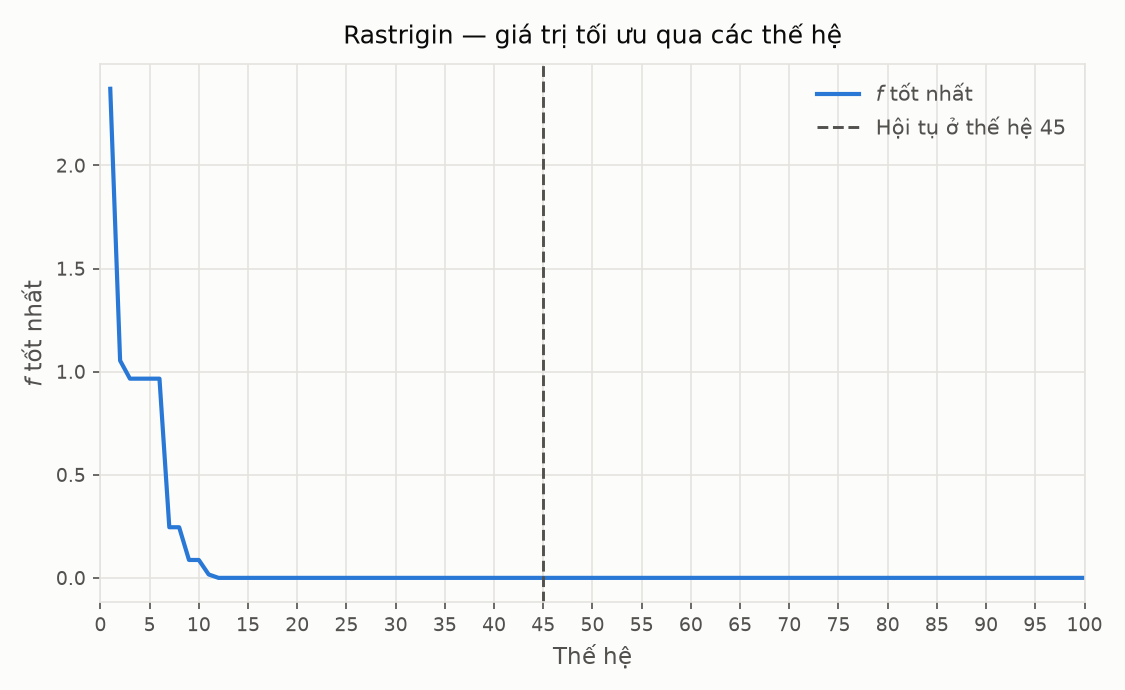
\includegraphics[width=\linewidth]{figures/hoitu_rastrigin.png}
    \caption{Đường hội tụ của GA}
\end{subfigure}
\caption{Hàm Rastrigin: mạng lưới cực tiểu cục bộ dày đặc quanh cực
tiểu toàn cục, và diễn biến giá trị tốt nhất qua các thế hệ.}
\label{fig:rastrigin}
\end{figure}

\textbf{Hàm Rosenbrock} có công thức
\begin{equation}
f(x,y) = (1-x)^2 + 100(y-x^2)^2,
\qquad x \in [-5,\, 10],\ y \in [-5,\, 10],
\label{eq:rosenbrock}
\end{equation}
với cực tiểu toàn cục $f(1,1) = 0$. Khác hẳn bốn hàm còn lại, hàm này
\textit{không} đa cực trị: trên miền hai biến nó chỉ có duy nhất một
cực tiểu, nên không tồn tại bẫy cục bộ nào để thuật toán mắc vào. Khó
khăn nằm ở hình dạng của đáy hàm. Số hạng $100(y-x^2)^2$ phạt rất nặng
mọi sai lệch khỏi đường cong $y = x^2$, tạo thành một thung lũng hẹp
hình quả chuối với vách hai bên dựng đứng, trong khi dọc theo lòng
thung lũng giá trị hàm lại thay đổi rất chậm. Muốn tiến về $(1,1)$,
thuật toán phải thay đổi $x$ và $y$ một cách \textit{phối hợp} sao cho
$y$ luôn bám theo $x^2$; đi lệch nhịp là lập tức đâm vào vách. Cụ thể,
để đạt được $f < 10^{-3}$ thì đồng thời phải có $|1-x| < 0{,}032$ và
$|y-x^2| < 0{,}0032$ --- một dải rất mỏng và cong. Cả hai toán tử của
GA đều không phù hợp với yêu cầu này: lai ghép trộn nội suy theo
\textit{đường thẳng} nối hai cha mẹ, còn đột biến Gauss xê dịch từng
tọa độ một cách \textit{độc lập}, nên không toán tử nào bám được theo
một đường cong. Nói cách khác, với Rosenbrock cái khó không phải là
\textit{tìm ra} vùng chứa nghiệm mà là \textit{dò theo} đáy thung lũng
sau khi đã vào được trong đó.

\begin{figure}[htbp]
\centering
\begin{subfigure}[b]{0.72\linewidth}
    \centering
    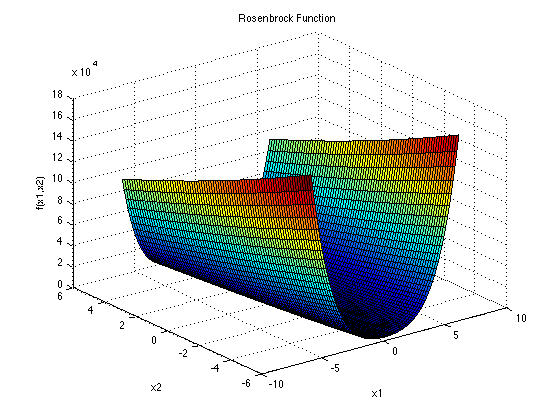
\includegraphics[width=\linewidth]{figures/rosenbrock.png}
    \caption{Hàm Rosenbrock trong không gian ba chiều}
\end{subfigure}

\vspace{0.8em}

\begin{subfigure}[b]{0.72\linewidth}
    \centering
    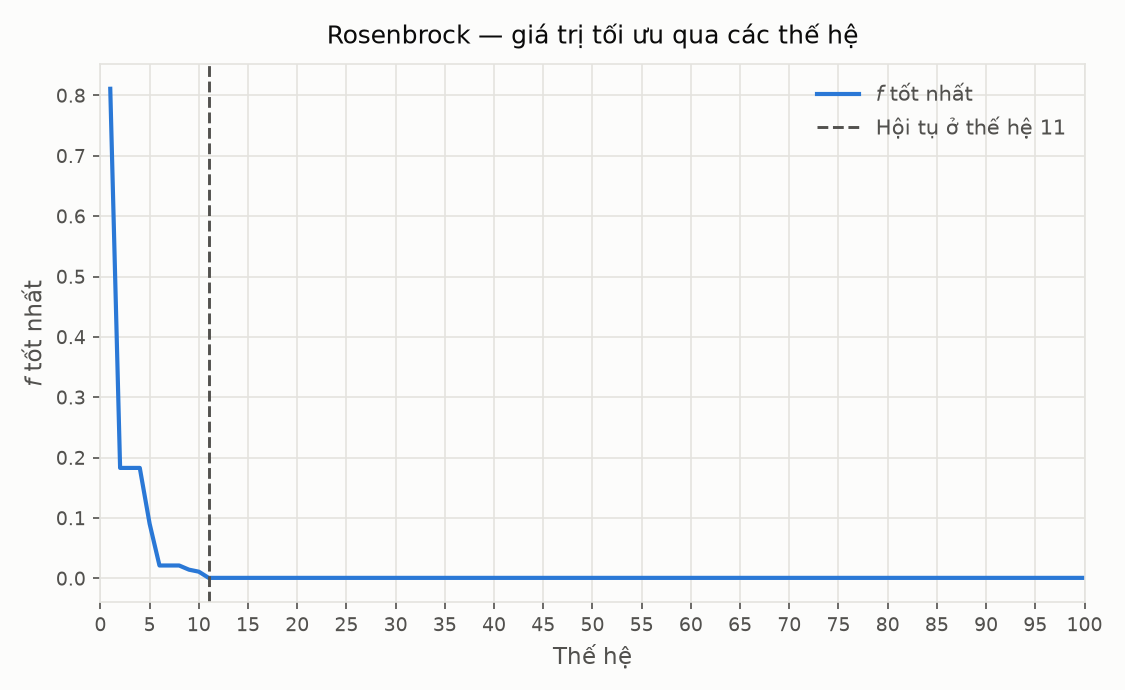
\includegraphics[width=\linewidth]{figures/hoitu_rosenbrock.png}
    \caption{Đường hội tụ của GA}
\end{subfigure}
\caption{Hàm Rosenbrock: thung lũng cong hẹp hình quả chuối, và diễn
biến giá trị tốt nhất qua các thế hệ --- GA chốt kỷ lục ngay ở thế hệ
$11$ rồi không cải thiện thêm trong $89$ thế hệ còn lại.}
\label{fig:rosenbrock}
\end{figure}

\textbf{Hàm Ackley} có công thức
\begin{equation}
\begin{split}
f(x,y) = {} & -20\exp\!\left(-0.2\sqrt{0.5(x^2+y^2)}\right) \\
& - \exp\!\left(0.5\cos(2\pi x) + 0.5\cos(2\pi y)\right) + 20 + e,
\end{split}
\label{eq:ackley}
\end{equation}
với $x, y \in [-32.768,\, 32.768]$ và cực tiểu toàn cục $f(0,0) = 0$.
Hàm này kết hợp hai cấu trúc chồng lên nhau ở hai thang độ khác nhau:
số hạng mũ thứ nhất tạo một cái phễu lớn dốc dần về gốc tọa độ, còn số
hạng cosin phủ lên bề mặt phễu đó vô số gợn sóng cực tiểu cục bộ nhỏ.
Cấu trúc phễu ở thang lớn là thông tin có ích --- nó chỉ đúng hướng
về nghiệm; các gợn sóng ở thang nhỏ mới là bẫy. Do đó Ackley kiểm tra
khả năng \textit{đọc được xu thế toàn cục mà không bị nhiễu cục bộ
đánh lạc hướng}. Với GA, biên độ đột biến
$\sigma = 0{,}08 \times 65{,}536 \approx 5{,}24$ lớn hơn nhiều so với
bước sóng của gợn nhiễu (bằng $1$), nên các gợn sóng gần như trong
suốt đối với quá trình tìm kiếm.

\begin{figure}[htbp]
\centering
\begin{subfigure}[b]{0.72\linewidth}
    \centering
    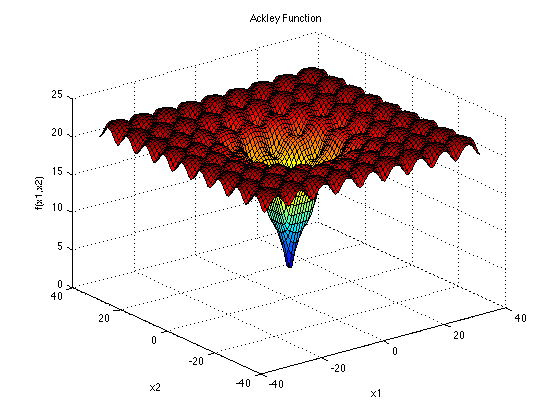
\includegraphics[width=\linewidth]{figures/ackley.png}
    \caption{Hàm Ackley trong không gian ba chiều}
\end{subfigure}

\vspace{0.8em}

\begin{subfigure}[b]{0.72\linewidth}
    \centering
    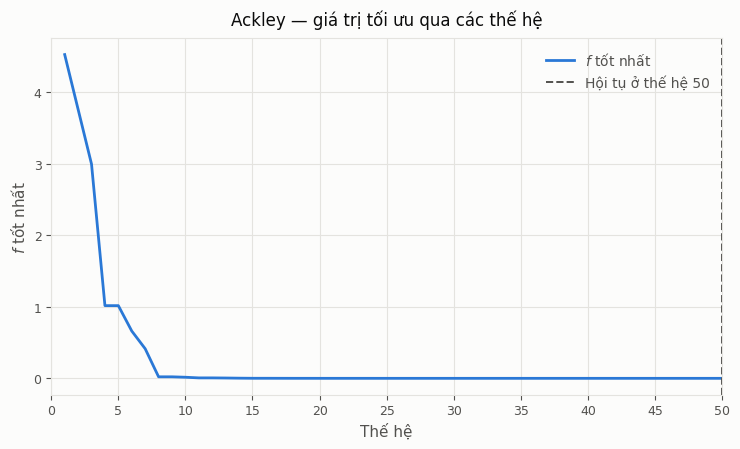
\includegraphics[width=\linewidth]{figures/hoitu_ackley.png}
    \caption{Đường hội tụ của GA}
\end{subfigure}
\caption{Hàm Ackley: phễu lớn ở thang toàn cục phủ gợn sóng cực tiểu
cục bộ ở thang nhỏ, và diễn biến giá trị tốt nhất qua các thế hệ.}
\label{fig:ackley}
\end{figure}

\textbf{Hàm Schwefel} có công thức
\begin{equation}
f(x,y) = 837.9658 - x\sin\sqrt{|x|} - y\sin\sqrt{|y|},
\qquad x, y \in [-500,\, 500],
\label{eq:schwefel}
\end{equation}
với cực tiểu toàn cục $f(420.9687,\, 420.9687) \approx 0$. Đây là hàm
được thiết kế để \textit{đánh lừa}: các cực tiểu cục bộ của nó phân bố
không đều, và điều nguy hiểm là cực tiểu cục bộ tốt thứ nhì lại nằm
rất xa cực tiểu toàn cục trong không gian tìm kiếm. Hệ quả là thông
tin cục bộ dẫn đường sai --- một thuật toán càng khai thác sớm và
càng mạnh vùng đang có vẻ tốt thì càng bị kéo ra xa nghiệm đúng. Thêm
vào đó, cực tiểu toàn cục nằm ở $420{,}97$, tức sát biên $500$ của
miền tìm kiếm, nên những cài đặt cắt hoặc co cá thể về phía tâm miền
sẽ bỏ sót nó. Hàm này vì vậy kiểm tra khả năng duy trì thăm dò trên
diện rộng và không cam kết quá sớm vào một vùng.

\begin{figure}[htbp]
\centering
\begin{subfigure}[b]{0.72\linewidth}
    \centering
    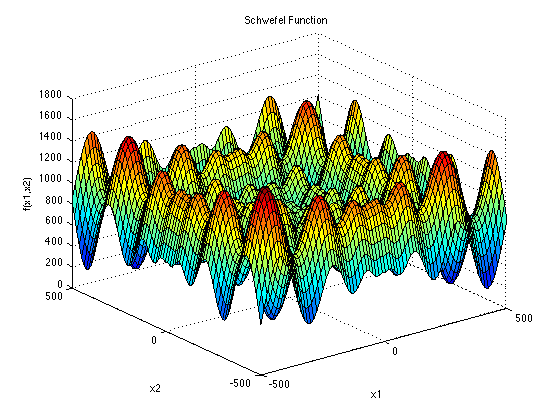
\includegraphics[width=\linewidth]{figures/schwefel.png}
    \caption{Hàm Schwefel trong không gian ba chiều}
\end{subfigure}

\vspace{0.8em}

\begin{subfigure}[b]{0.72\linewidth}
    \centering
    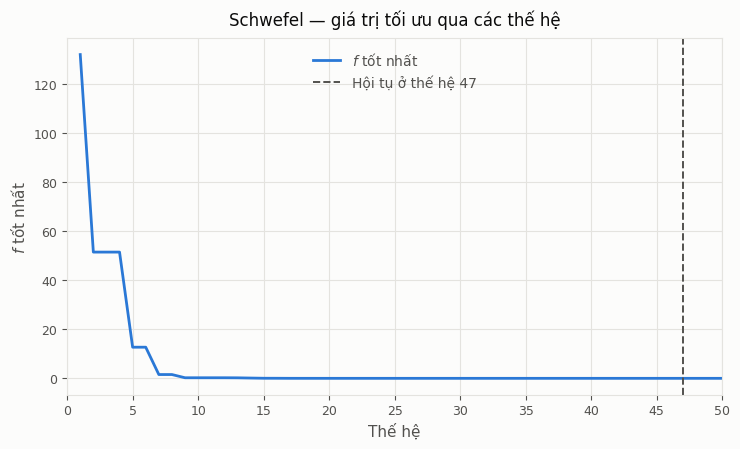
\includegraphics[width=\linewidth]{figures/hoitu_schwefel.png}
    \caption{Đường hội tụ của GA}
\end{subfigure}
\caption{Hàm Schwefel: cực tiểu toàn cục nằm gần biên miền tìm kiếm,
xa vùng trông có vẻ tốt quanh gốc tọa độ, và diễn biến giá trị tốt
nhất qua các thế hệ.}
\label{fig:schwefel}
\end{figure}

Với mỗi hàm, GA mã hóa số thực (lai ghép trộn BLX-$\alpha$ với
$\alpha \in [-0{,}25;\, 1{,}25]$, đột biến Gauss với xác suất $0{,}15$
trên mỗi gene và $\sigma$ bằng $0{,}08$ lần bề rộng miền, chọn lọc
giải đấu theo thứ hạng với $k = 3$, giữ lại $2$ cá thể tinh hoa mỗi
thế hệ --- theo Mục~\ref{sec:toan-tu-cot-loi}) được chạy một lần với
quần thể $500$ cá thể trong $100$ thế hệ, hạt giống ngẫu nhiên cố định
bằng $42$ để kết quả tái lập được. Cá thể được cắt về miền tìm kiếm
sau mỗi phép lai ghép và đột biến, vì ở đây miền đóng vai trò miền xác
định của bài toán. Thuật toán không có tiêu chí dừng sớm: vòng lặp
luôn chạy đủ $100$ thế hệ. Cột \textit{số thế hệ thỏa mãn} trong
Bảng~\ref{tab:kq-khong-rang-buoc} vì vậy không phải thế hệ mà thuật
toán dừng lại, mà là thế hệ sớm nhất đạt được giá trị $f^{*}$ cuối
cùng --- tức lần cuối cùng kỷ lục được cải thiện.

\begin{table}[htbp]
\centering
\caption{Kết quả GA trên năm hàm benchmark không ràng buộc}
\label{tab:kq-khong-rang-buoc}
\small
\setlength{\tabcolsep}{5pt}
\begin{tabular}{lccccc}
\toprule
\textbf{Hàm} & \textbf{Thời gian} & \textbf{Số thế hệ}
& \textbf{$f^{*}$} & \textbf{$x^{*}$} & \textbf{$y^{*}$} \\
& \textbf{(s)} & \textbf{thỏa mãn} & & & \\
\midrule
Easom      & $1.3619$ & $51$ & $-1.0000000000$      & $3.141593$              & $3.141593$               \\
Rastrigin  & $1.3876$ & $45$ & $0.0000000000$       & $8.00\times10^{-10}$    & $-2.11\times10^{-9}$     \\
Rosenbrock & $1.4194$ & $11$ & $0.0009051359$       & $1.008839$              & $1.014881$               \\
Ackley     & $1.5411$ & $76$ & $0.0000000000$       & $-9.22\times10^{-17}$   & $-2.99\times10^{-16}$    \\
Schwefel   & $1.4160$ & $52$ & $2.5455\times10^{-5}$ & $420.968746$           & $420.968746$             \\
\bottomrule
\end{tabular}
\end{table}

GA tìm đúng, hoặc gần đúng đến sai số không đáng kể, cực tiểu toàn cục
trên cả năm hàm --- kể cả Easom và Schwefel, hai hàm được thiết kế
riêng để đánh lừa các thuật toán chỉ khai thác thông tin cục bộ quanh
điểm hiện tại. Kết quả này minh chứng trực tiếp cho ưu điểm cốt lõi
của tìm kiếm dựa trên quần thể đã trình bày ở
Mục~\ref{subsec:ho-thuat-toan-tien-hoa}: vì GA duy trì $500$ cá thể
trải rộng trên không gian tìm kiếm thay vì một điểm duy nhất, nó không
phụ thuộc vào việc điểm khởi tạo có nằm gần cực tiểu toàn cục hay
không, khác với các phương pháp gradient cổ điển. Với Rastrigin và
Ackley, GA về đúng $0$ trong giới hạn biểu diễn số thực dấu phẩy động.

Rosenbrock là ngoại lệ duy nhất, và cách nó khác biệt lại soi sáng
đúng điểm mạnh cũng như điểm yếu của GA. Sai số $9{,}05\times10^{-4}$
của nó lớn hơn bốn hàm còn lại nhiều bậc độ lớn, mặc dù đây là hàm
\textit{duy nhất} trong năm hàm không hề có bẫy cực tiểu cục bộ.
Đường hội tụ ở Hình~\ref{fig:rosenbrock} cho thấy rõ cơ chế: giá trị
tốt nhất tụt rất nhanh trong mười thế hệ đầu rồi chốt lại ở thế hệ
$11$ và đứng yên suốt $89$ thế hệ còn lại. Nghĩa là GA lọt vào đúng
thung lũng gần như tức thì, nhưng sau đó không nhích thêm được nữa.
Đối chiếu với Ackley --- hàm mà GA cải thiện kỷ lục rải rác cho tới
tận thế hệ $76$ --- có thể thấy hai kiểu khó khăn hoàn toàn khác nhau:
Rastrigin, Ackley, Easom và Schwefel khó ở chỗ \textit{tìm ra} đúng
vùng chứa nghiệm, còn Rosenbrock khó ở chỗ \textit{dò theo} một cấu
trúc cong sau khi đã tìm ra vùng đó.

Sự phân đôi này phản ánh bản chất của các toán tử tiến hóa ngẫu nhiên
đẳng hướng: chúng rất mạnh trong việc định vị một vùng rộng trên không
gian tìm kiếm, nhưng yếu trong việc tinh chỉnh dọc theo một hướng ưu
tiên hẹp. Đây chính là lý do các thuật toán lai ghép GA với tìm kiếm
cục bộ (memetic algorithm) tồn tại --- và cũng là cách tiếp cận được
áp dụng cho bài toán người du lịch ở Mục~\ref{sec:ud-tsp}, nơi GA
thuần túy được bổ sung thêm bước tối ưu cục bộ 2-opt để xử lý đúng
phần việc mà lai ghép và đột biến ngẫu nhiên làm không tốt.

\section{Tối ưu có ràng buộc: So sánh GA với SciPy SLSQP}
\label{sec:ud-co-rang-buoc}

Năm bài toán tối ưu có ràng buộc được lựa chọn để bao quát các dạng
ràng buộc và tính chất hàm mục tiêu khác nhau, từ tuyến tính tuyệt đối
đến phi tuyến.

\textbf{Bài toán 1 — Entropy tối đa.} Đây là bài toán ``con xúc xắc bị
làm lệch'' của Jaynes: tìm phân phối xác suất $x_1,\ldots,x_6$ của một
con xúc xắc sáu mặt có entropy lớn nhất, biết trước kỳ vọng
$E[X]=4.5$. Sau khi đổi dấu để đưa về bài toán cực tiểu hóa (vì
$\max H(x) \equiv \min -H(x)$), phát biểu toán học là
\begin{equation}
\min_{x \in \mathbb{R}^6} f(x) = \sum_{i=1}^{6} x_i \ln x_i
\quad \text{s.t.} \quad
\sum_{i=1}^{6} x_i = 1,\quad
\sum_{i=1}^{6} i\, x_i = 4.5,\quad
x_i \ge 0.
\label{eq:entropy}
\end{equation}
Hai ràng buộc đẳng thức phải được thỏa mãn đồng thời, khiến miền khả
thi chỉ còn là giao tuyến của hai siêu phẳng trong $\mathbb{R}^6$.

\textbf{Bài toán 2 — Điểm gần nhất trong miền ràng buộc.} Cho một điểm
$(5,\, 4,\, -2)$ nằm ngoài miền ràng buộc, tìm điểm $(x,y,z)$ trong
miền ràng buộc gần điểm đó nhất theo khoảng cách Euclid bình phương —
tức là bài toán chiếu một điểm lên một tập lồi:
\begin{equation}
\min_{x,y,z} f(x,y,z) = (x-5)^2+(y-4)^2+(z+2)^2
\quad \text{s.t.} \quad
x+2y+z=4,\quad
x^2+y^2\le9,\quad
z\ge0.
\label{eq:nearest-point}
\end{equation}
Miền ràng buộc là giao của một mặt phẳng, một hình trụ, và một nửa
không gian.

\textbf{Bài toán 3 — Quy hoạch tuyến tính.} Hàm mục tiêu và mọi ràng
buộc đều tuyến tính:
\begin{equation}
\max_{x,y,z} f(x,y,z) = 3x+5y-2z
\quad \text{s.t.} \quad
x+2y+z=10,\quad
2x+y\le8,\quad
x,y,z\ge0.
\label{eq:lp}
\end{equation}
Vì là quy hoạch tuyến tính (LP) thuần túy, nghiệm tối ưu chắc chắn nằm
tại một đỉnh của miền đa diện lồi xác định bởi các ràng buộc.

\textbf{Bài toán 4 — Quy hoạch bình phương.} Hàm mục tiêu bậc hai lồi,
ràng buộc tuyến tính:
\begin{equation}
\min_{x,y,z} f(x,y,z) = x^2+2y^2+z^2-4x-6y
\quad \text{s.t.} \quad
x+y+2z=5,\quad
x+y\le3,\quad
x,y,z\ge0.
\label{eq:qp}
\end{equation}
Vì hàm mục tiêu lồi và miền ràng buộc lồi, bài toán này (quy hoạch
bình phương — QP) có đúng một cực tiểu toàn cục.

\textbf{Bài toán 5 — Tối ưu lồi phi tuyến.} Hàm mục tiêu là tổng hai
hàm mũ, khác hẳn tính chất tuyến tính từng khúc của bốn bài toán trên:
\begin{equation}
\min_{x,y} f(x,y) = e^{-x}+e^{-2y}
\quad \text{s.t.} \quad
2x+3y=6,\quad
x^2+y^2\le4,\quad
x,y\ge0.
\label{eq:convex-exp}
\end{equation}
Cả hàm mục tiêu lẫn miền ràng buộc đều lồi nên bài toán vẫn có đúng
một cực tiểu toàn cục, dù không còn là dạng tuyến tính hay bình phương.

GA cho cả năm bài toán này sử dụng chiến lược xử lý ràng buộc đã giới
thiệu ở Mục~\ref{subsec:ham-thich-nghi} — kết hợp quy tắc khả thi Deb
với ngưỡng $\varepsilon$ giảm dần theo thời gian, thay vì hàm phạt
tĩnh — chạy với quần thể $1000$ cá thể trong tối đa $500$ thế hệ, lặp
lại ba lần độc lập. Đối trọng so sánh là SciPy SLSQP, một phương pháp
tối ưu dựa trên gradient giải theo điều kiện KKT, được chạy từ $30$
điểm khởi tạo ngẫu nhiên khác nhau để giảm rủi ro hội tụ về một cực
tiểu cục bộ thay vì cực tiểu toàn cục. Kết quả tốt nhất của mỗi phương
pháp được trình bày ở Bảng~\ref{tab:kq-co-rang-buoc}.

\begin{table}[htbp]
\centering
\caption{Kết quả GA và SciPy SLSQP trên năm bài toán tối ưu có ràng buộc}
\label{tab:kq-co-rang-buoc}
\begin{tabular}{lcc}
\toprule
\textbf{Bài toán} & \textbf{GA ($f^{*}$)} & \textbf{SLSQP ($f^{*}$)} \\
\midrule
1. Entropy tối đa            & $-1.5985825694$  & $-1.6135810982$ \\
2. Điểm gần nhất             & $20.3497958340$  & $20.2756044350$ \\
3. Quy hoạch tuyến tính (LP) & $-25.9149581523$ & $-26.0000000000$ \\
4. Quy hoạch bình phương (QP)& $-7.3329937494$  & $-7.3333333333$ \\
5. Tối ưu lồi phi tuyến      & $0.3565975317$   & $0.3565154830$  \\
\bottomrule
\end{tabular}
\end{table}

SLSQP đạt kết quả nhỉnh hơn GA một chút ở cả năm bài toán. Điều này
đúng như kỳ vọng lý thuyết, vì cả năm bài toán đều lồi và có hàm mục
tiêu khả vi — chính là điều kiện lý tưởng nhất cho một phương pháp dựa
trên gradient và điều kiện KKT như SLSQP, trong khi GA không khai thác
được thông tin đạo hàm này để tinh chỉnh nghiệm ở bước cuối. Tuy vậy,
khoảng cách giữa hai phương pháp rất nhỏ: GA đạt trong khoảng
$0.01\%$ đến $1\%$ so với SLSQP ở bốn trong năm bài toán; riêng bài
toán 3 (LP) có sai số tương đối lớn hơn một chút, vì nghiệm tối ưu của
LP luôn nằm đúng tại một đỉnh sắc cạnh của miền đa diện — một điểm mà
các toán tử lai ghép/đột biến liên tục của GA khó tiệm cận chính xác
tuyệt đối hơn so với việc dò theo một đường cong trơn. Nhìn chung, kết
quả cho thấy GA vẫn xấp xỉ tốt cả năm bài toán dù không dùng đến đạo
hàm. Điều này có ý nghĩa thực tiễn quan trọng: trong các bài toán mà
hàm mục tiêu không khả vi hoặc không lồi — nơi SLSQP không còn đảm bảo
hội tụ đúng — khả năng xấp xỉ tốt của GA mà không cần thông tin đạo
hàm trở thành một lợi thế thực sự, như sẽ thấy rõ hơn ở hai bài toán
tiếp theo.

\section{Bài toán Người du lịch: GA hoán vị kết hợp Tìm kiếm Cục bộ}
\label{sec:ud-tsp}

Bài toán người du lịch (Traveling Salesman Problem — TSP) được phát
biểu như sau: cho $n$ địa điểm và ma trận khoảng cách
$D = (d_{ij})_{n\times n}$ giữa mọi cặp địa điểm, tìm một hoán vị
$\pi = (\pi_1, \ldots, \pi_n)$ của $n$ địa điểm sao cho tổng độ dài lộ
trình khép kín đi qua tất cả các địa điểm đúng một lần là nhỏ nhất:
\begin{equation}
\min_{\pi} L(\pi) = \sum_{k=1}^{n-1} d_{\pi_k, \pi_{k+1}} + d_{\pi_n, \pi_1}.
\label{eq:tsp}
\end{equation}
Bài toán này được mã hóa dưới dạng hoán vị đã giới thiệu ở
Mục~\ref{subsec:ma-hoa}: mỗi cá thể của GA chính là một hoán vị $\pi$,
dùng lai ghép Order Crossover (OX) và đột biến Swap (Mục~\ref{sec:toan-tu-cot-loi})
thay cho các toán tử số thực ở hai mục trước.

Để đánh giá khách quan trên dữ liệu thực thay vì các ví dụ tự tạo quy
mô nhỏ, ba bộ dữ liệu chuẩn từ thư viện benchmark TSPLIB95 [9] được sử
dụng: berlin52 ($n=52$ địa điểm tại Berlin), rd100 ($n=100$ địa điểm
ngẫu nhiên), và ch150 ($n=150$ địa điểm). Mỗi bộ dữ liệu đều có kèm
theo lộ trình tối ưu đã được công bố, dùng làm mốc đối chiếu khách
quan thay cho phương pháp vét cạn — vốn cần thử $(n-1)!$ hoán vị và
trở nên bất khả thi về mặt tính toán ngay từ $n$ vài chục.

Thử nghiệm ban đầu với GA hoán vị thuần túy (chỉ dùng OX và Swap) cho
kết quả chênh lệch rất lớn so với nghiệm tối ưu đã công bố, từ $20\%$
đến $84\%$ tùy bộ dữ liệu và tăng dần theo số địa điểm $n$. Nguyên
nhân là hai toán tử OX và Swap không có cơ chế sửa các đoạn đường bị
cắt chéo nhau trong lộ trình — một lộ trình càng có nhiều địa điểm thì
càng dễ chứa những đoạn cắt chéo như vậy, và OX/Swap chỉ có thể tạo ra
một cấu hình mới ngẫu nhiên chứ không chủ động ``gỡ'' đoạn cắt chéo đó.
Để khắc phục hạn chế này, một chiến lược lai giữa GA và tìm kiếm cục bộ
(\textit{memetic algorithm}) được áp dụng: sau mỗi thế hệ, một tỉ lệ cá
thể tốt nhất trong quần thể được tinh chỉnh thêm bằng phép tìm kiếm cục
bộ \textbf{2-opt} — xét lần lượt từng cặp cạnh trong lộ trình, hoán đổi
hai cạnh đó nếu việc hoán đổi làm giảm tổng độ dài — trước khi tiếp tục
vòng lặp tiến hóa (chọn lọc, lai ghép, đột biến) như bình thường. Với
tỉ lệ tinh chỉnh bằng khoảng $5\%$ quần thể mỗi thế hệ, cả ba bộ dữ
liệu đều đạt đúng lộ trình tối ưu đã công bố, như trình bày ở
Bảng~\ref{tab:kq-tsp}.

\begin{table}[htbp]
\centering
\caption{Kết quả GA kết hợp 2-opt trên ba bộ dữ liệu TSPLIB95}
\label{tab:kq-tsp}
\begin{tabular}{lcccc}
\toprule
\textbf{Bộ dữ liệu} & \textbf{Số địa điểm ($n$)} & \textbf{Nghiệm tối ưu} & \textbf{GA} & \textbf{Đạt được ở thế hệ} \\
\midrule
berlin52 & 52  & 7542 & 7542 & 8/50  \\
rd100    & 100 & 7910 & 7910 & 48/50 \\
ch150    & 150 & 6528 & 6528 & 37/50 \\
\bottomrule
\end{tabular}
\end{table}

Trong quá trình hiệu chỉnh tham số, một quan sát quan trọng được ghi
nhận: tỉ lệ cá thể được tinh chỉnh bằng 2-opt cần được đặt theo
\textit{phần trăm} của quần thể chứ không phải theo một số lượng cố
định. Cụ thể, khi giữ nguyên số lượng cá thể được tinh chỉnh ở một
con số tuyệt đối nhưng tăng kích thước quần thể lên, kết quả trở nên
tệ hơn so với quần thể nhỏ — nguyên nhân là vì trong một quần thể lớn,
số cá thể đã qua tinh chỉnh chiếm tỉ lệ quá nhỏ nên khó lan gen tốt ra
phần còn lại của quần thể thông qua phép chọn lọc. Quan sát này cho
thấy các tham số của một chiến lược lai giữa GA và tìm kiếm cục bộ
không thể được chọn độc lập với nhau, mà phải cân chỉnh tương thích
với quy mô quần thể.

\section{Hồi quy Ký hiệu bằng Lập trình Di truyền}
\label{sec:ud-symbolic-regression}

Ứng dụng cuối cùng minh họa Lập trình Di truyền (Mục~\ref{sec:gp}) cho
bài toán hồi quy ký hiệu trên dữ liệu vật lý thực: các phép đo mật độ
hạt, vận tốc, và từ trường của gió mặt trời do vệ tinh WIND của NASA
ghi nhận. Ba thành phần từ trường đo được là $B_X, B_Y, B_Z$, và mật độ
hạt đo được là $n$. Từ bốn đại lượng này, hai đại lượng vật lý phái
sinh được chọn làm mục tiêu dự đoán cho GP:
\begin{equation}
|B|^2 = B_X^2+B_Y^2+B_Z^2
\qquad \text{(bình phương độ lớn từ trường)},
\label{eq:b-squared}
\end{equation}
\begin{equation}
V_A^2 \propto \frac{|B|^2}{n}
\qquad \text{(vận tốc Alfvén bình phương)}.
\label{eq:alfven-squared}
\end{equation}
Đại lượng thứ nhất là một quan hệ tổng bình phương (dạng Pythagore)
giữa ba biến đo được; đại lượng thứ hai kết hợp thêm một phép chia cho
biến mật độ hạt.

Điểm mấu chốt khiến hai đại lượng này trở thành phép thử công bằng cho
GP là: quan hệ tổng bình phương ở Phương trình~\eqref{eq:b-squared}
\textit{không thể} tuyến tính hóa bằng phép biến đổi logarit như các
quan hệ dạng lũy thừa thông thường, vì $B_X, B_Y, B_Z$ có thể mang giá
trị âm nên không lấy logarit được. Do đó, Hồi quy Tuyến tính áp dụng
trực tiếp trên ba đặc trưng thô $B_X, B_Y, B_Z$ gần như chắc chắn
không thể biểu diễn được cấu trúc bậc hai này, vì mô hình tuyến tính
chỉ có thể biểu diễn một tổ hợp tuyến tính của chính các đặc trưng đó,
không tự sinh ra được số hạng bậc hai. Ngược lại, GP có thể tự xây
dựng số hạng bậc hai bằng cách nhân một biến với chính nó ngay trong
cây biểu thức, mà không cần được cung cấp trước các đặc trưng
$B_X^2, B_Y^2, B_Z^2$ như một phép biến đổi thủ công. Kết quả đối
chiếu hai phương pháp trên tập kiểm tra được trình bày ở
Bảng~\ref{tab:kq-symbolic-regression}.

\begin{table}[htbp]
\centering
\caption{Kết quả Hồi quy Tuyến tính và GP trên hai đại lượng vật lý phái sinh}
\label{tab:kq-symbolic-regression}
\begin{tabular}{llccc}
\toprule
\textbf{Đại lượng} & \textbf{Phương pháp} & \textbf{MAE} & \textbf{RMSE} & \textbf{$R^2$} \\
\midrule
\multirow{2}{*}{$|B|^2$}
    & Hồi quy Tuyến tính & 15.1284 & 19.9825 & 0.4784 \\
    & GP (hồi quy ký hiệu) & 4.1820 & 6.0779 & 0.9517 \\
\addlinespace
\multirow{2}{*}{$V_A^2$}
    & Hồi quy Tuyến tính & 2.7376 & 3.6804 & 0.4629 \\
    & GP (hồi quy ký hiệu) & 1.0554 & 1.5486 & 0.9049 \\
\bottomrule
\end{tabular}
\end{table}

Kết quả cho thấy chênh lệch rõ rệt và nhất quán trên cả hai đại lượng.
Hồi quy Tuyến tính chỉ giải thích được khoảng $46\%$ đến $48\%$ phương
sai của dữ liệu ($R^2 \approx 0.46$–$0.48$), trong khi GP đạt trên
$90\%$ ($R^2 \approx 0.90$–$0.95$); đồng thời sai số dự đoán (MAE,
RMSE) của GP chỉ còn chưa đến một phần ba so với Hồi quy Tuyến tính ở
cả hai đại lượng. Đây là kết quả trái ngược hẳn với các bài toán hồi
quy dạng lũy thừa từng được thử nghiệm trong quá trình thực hiện tiểu
luận — ví dụ định luật Kepler III hay áp suất động của gió mặt trời —
là những quan hệ trở thành tuyến tính tuyệt đối sau khi biến đổi
logarit, khiến Hồi quy Tuyến tính ở các bài toán đó luôn đạt hoặc vượt
GP. Sự tương phản giữa hai nhóm kết quả khẳng định đúng giả thuyết ban
đầu: lợi thế thực sự của GP so với hồi quy cổ điển chỉ bộc lộ rõ khi
quan hệ cần khám phá có cấu trúc phi tuyến mà phép biến đổi đặc trưng
thủ công thông thường, như logarit, không xử lý được.

\section{Tổng kết Chương}
\label{sec:ud-tong-ket}

Bốn thực nghiệm trên minh họa một đặc điểm xuyên suốt của Thuật toán
Di truyền: tính linh hoạt cao nhờ khả năng thích ứng với nhiều cách mã
hóa khác nhau — số thực ở Mục~\ref{sec:ud-khong-rang-buoc}
và~\ref{sec:ud-co-rang-buoc}, hoán vị ở Mục~\ref{sec:ud-tsp}, và cây
biểu thức ở Mục~\ref{sec:ud-symbolic-regression}. Đổi lại tính linh
hoạt đó là hiệu quả thấp hơn các phương pháp chuyên dụng khi bài toán
có sẵn một cấu trúc mà phương pháp đó khai thác được: SLSQP khai thác
tính khả vi và tính lồi của năm bài toán ở
Mục~\ref{sec:ud-co-rang-buoc}. Ngược lại, ở những bài toán mà cấu trúc
đó không có sẵn, hoặc phương pháp cổ điển tương ứng không còn đủ mạnh
— bài toán người du lịch quy mô lớn cần bổ sung tìm kiếm cục bộ mới
đạt được nghiệm tối ưu, hay quan hệ phi tuyến dạng tổng bình phương mà
Hồi quy Tuyến tính không thể biểu diễn được — GA và GP thể hiện rõ giá
trị thực tiễn của một phương pháp tìm kiếm không đặt giả định trước về
cấu trúc bài toán.
